\begin{multicols}{3}
\begin{Figure}
 \centering
 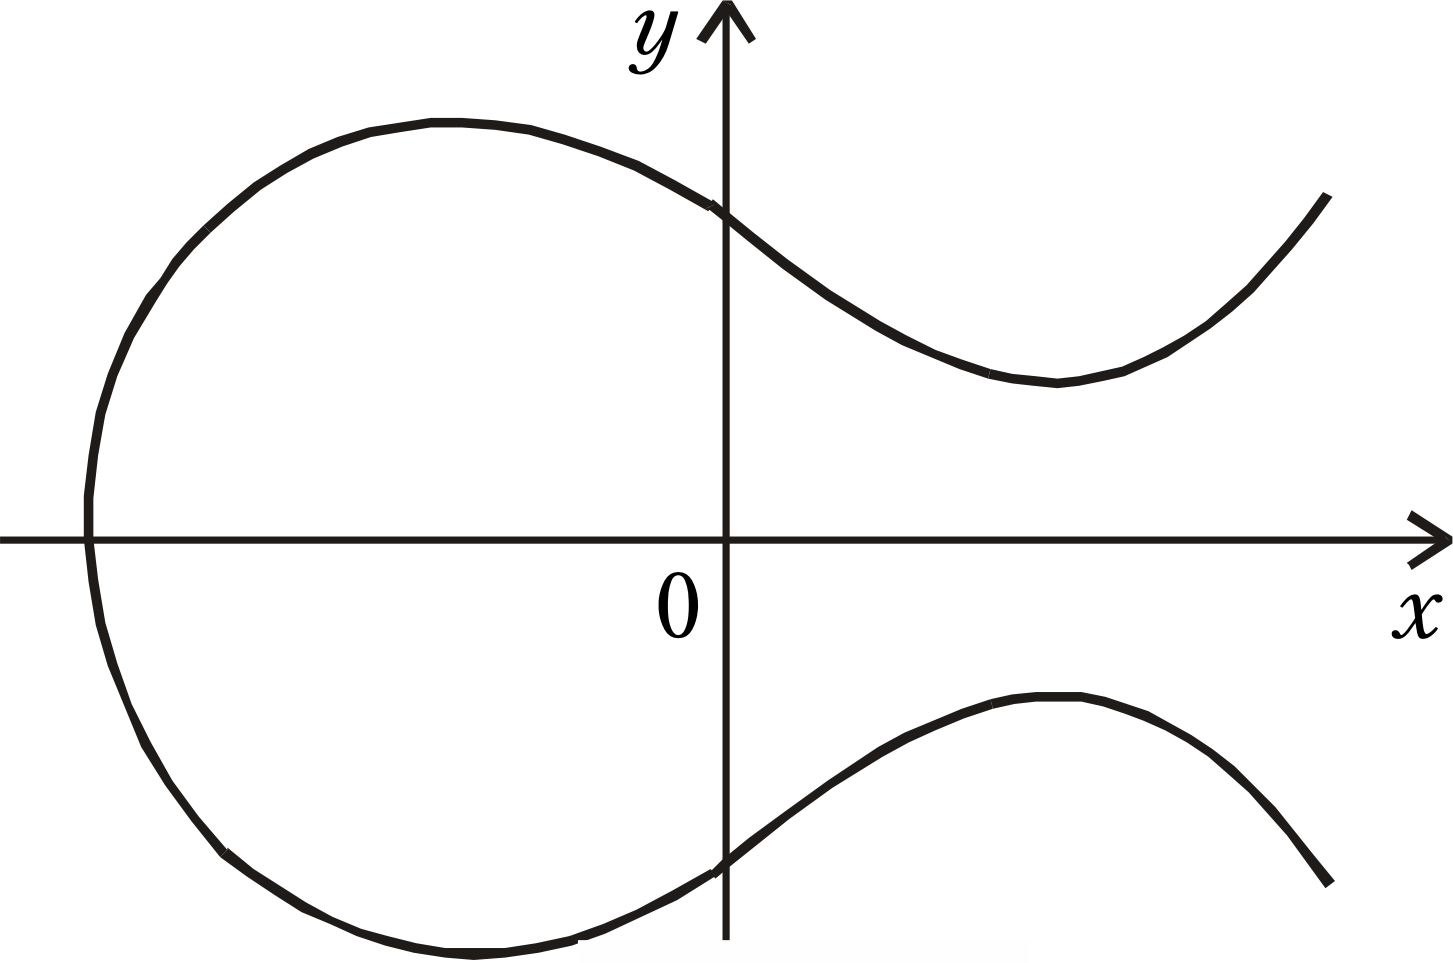
\includegraphics[width=\columnwidth]{fig1}
 \captionof{figure}{}
 \hspace{\columnwidth}
 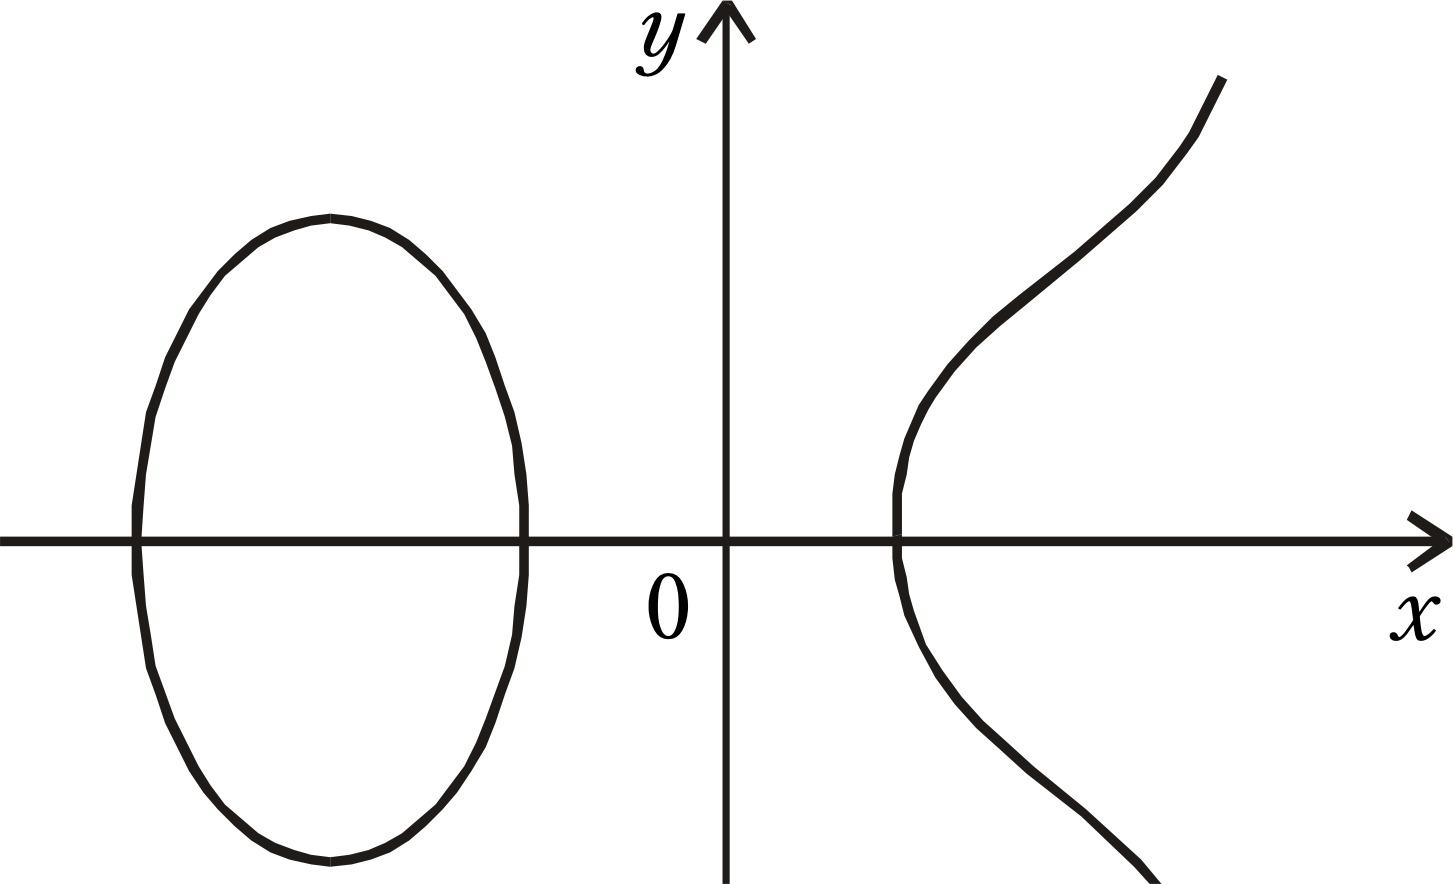
\includegraphics[width=\columnwidth]{fig2}
 \captionof{figure}{}
\end{Figure}
\noindent
Для кривой, заданной в канонической форме (2), дискриминант $\Delta$ определяется формулой
\begin{equation*}
    \Delta = -(4a^3 + 27b^2).
\end{equation*}
Пусть $E$  -- некоторая эллиптическая кривая, заданная уравнением
\begin{equation*}
    y^2 = x^3 + ax + b,
\end{equation*}
в котором $a$ и $b$ -- целые числа. Для простого числа $p$ рассмотрим сравнение
\begin{equation}
    \tag{3}
    \label{eq:comp}
    y^2 \equiv x^3 + \bar{a}x + \bar{b}\Mod{p},
\end{equation}
где $\bar{a}$ и $\bar{b}$ –- остатки от деления целых чисел $a$ и $b$ на $p$, и обозначим через $n_p$ число решений этого сравнения. Числа $n_p$ очень полезны при исследовании вопроса о разрешимости уравнений вида (2) в целых числах: если какое-то $n_p$ равно нулю, то уравнение (2) не имеет целочисленных решений. Однако вычислить числа $n_p$ удается лишь в редчайших случаях.
В то же время известно, что $|p - n_p| \leq 2 \sqrt{p}$ (теорема Хассе).

Рассмотрим те простые числа  $p$, которые делят дискриминант $\Delta $ эллиптической кривой (2). Можно доказать, что для таких $p$ многочлен $x^3 +\bar{a}x + \bar{b}$ можно записать одним из двух способов:
\begin{equation*}
    x^3 + \bar{a}x + \bar{b} \equiv (x + \bar{\alpha})^2(x + \bar{\beta})\Mod{p}
\end{equation*}
или
\begin{equation*}
    x^3 + \bar{a}x + \bar{b} \equiv (x + \bar{\gamma})^3\Mod{p},
\end{equation*}
где $\bar{\alpha}$, $\bar{\beta}$, $\bar{\gamma}$ -- некоторые остатки от деления на $p$. Если для всех простых $p$, делящих дискриминант кривой, реализуется первая из двух указанных возможностей, то эллиптическая кривая называется \emph{полустабильной}.

Простые числа, делящие дискриминант, можно объединить в так называемый \emph{кондуктор} эллиптической кривой. Если $E$ -- полустабильная кривая, то ее кондуктор $N$ задается формулой
\begin{equation}
    \tag{4}
    N = \prod_{p|\Delta}^{} p^{\varepsilon_p},
\end{equation}
где для всех простых чисел $p \geq 5$, делящих $\Delta$, показатель $\varepsilon_p$ равен $1$. Показатели $\varepsilon_2$ и $\varepsilon_3$ вычисляются с помощью специального алгоритма.
\subsection*{Модулярные формы и модулярные эллиптические кривые}

Обозначим через $H$ верхнюю комплексную полуплоскость. Пусть $N$ -- натуральное и $k$ -- целое числа. \emph{Модулярной параболической формой} веса $k$ уровня $N$ называется аналитическая функция $f(z)$, заданная в верхней полуплоскости и удовлетворяющая соотношению
\begin{equation}
    \tag{5}
    \label{eq:cond}
    f\left(\frac{az + b}{cz + b}\right) = (cz + d)^kf(z)
\end{equation}
для любых целых чисел $a$, $b$, $c$, $d$ таких, что $ad - bc = 1$ и $c$ делится на $N$. Кроме того, предполагается, что
\begin{equation*}
    \lim_{t\to+0} f(r + it) = 0,
\end{equation*}
где $r$ -- рациональное число, и что
\begin{equation*}
    \lim_{t\to\infty
    } f(it) = 0.
\end{equation*}

Пространство модулярных параболических форм веса $k$ уровня $N$ обозначается через $S_k(N)$. Можно показать, что оно имеет конечную размерность.

В дальнейшем нас будут особо интересовать модулярные параболические формы веса $2$. Для малых $N$ размерность $\dim S_2(N)$ пространства $S_2(N)$ представлена в таблице:
\begin{center}
\renewcommand{\arraystretch}{2}
\scalebox{0.85}{
  \begin{tabular}{ | c | c | c | c | c | c | c | }
    \hline
    $N < 10$ & 11 & 12 & 13 & 14 & 15 & 16 \\ \hline
    0 & 1 & 0 & 0 & 1 & 1 & 0 \\ \hline
     & 17 & 18 & 19 & 20 & 21 & 22 \\ \cline{2-7}
     & 1 & 0 & 1 & 1 & 1 & 2 \\
    \hline
  \end{tabular}}
\renewcommand{\arraystretch}{1}
\end{center}
В частности,
\begin{equation}
    \tag{6}
    \dim S_2(2) = 0.
\end{equation}

Отметим, что эта нехитрая формула сыграет важную роль в доказательстве теоремы Ферма.

Из условия \eqref{eq:cond} следует, что $f(z + 1) = f(z)$ для каждой формы $f \in S_2(N)$. Стало быть, $f$ является периодической функцией. Такую функцию можно представить в виде
\begin{equation}
    \tag{7}
    \label{eq:ser}
    f(z) = \sum_{n=1}^{\infty} a_nq^n, q = e^{2\pi iz}.
\end{equation}

Назовем модулярную параболическую форму $f(z) \in S_2(N)$ \emph{собственной}, если ее коэффициенты -- целые числа, удовлетворяющие соотношениям
\begin{equation*}
    a_1 = 1;
\end{equation*}
$a_{p^r}a_p = a_{p^{r+1}}pc_{p^{r-1}}$ для простого $p$, не делящего число $N$; (8)
\begin{equation*}
    a_{mn} = a_ma_n, \text{ если } (m, n) = 1.
\end{equation*}

Сформулируем теперь определение, играющее ключевую роль в доказательстве теоремы Ферма. Эллиптическая кривая с рациональными коффициентами и кондуктором $N$ называется \emph{модулярной}, если найдется такая собственная форма
\begin{equation}
    \tag{9}
    f(z) = \sum_{n=1}^{\infty} a_nq^n \in S_2(N),
\end{equation}
что $a_p = p - n_p$ для почти всех простых чисел $p$. Здесь $n_p$ 0 -- число решений сравнения \eqref{eq:comp}.
\subsection*{Гипотеза Таниямы}
\noindent
Определение модулярной эллиптической кривой является настолько жестким, что на первый взгляд кажется невероятным существование хотя бы одной такой кривой. Трудно представить, что функция $f(z)$, удовлетворяющая перечисленным выше весьма ограничительным условиям \eqref{eq:cond} и (8), разлагается в ряд \eqref{eq:ser}, коэффициенты которого связаны с практически невычислимыми числами $n_p$. Однако эмпирический материал, полученный в первой половине нашего века, позволил японскому математику Ю. Танияме (1927–1958) сформулировать в 1955 году удивительную гипотезу.
\end{multicols}
